\section{Experimental Setup}



We consider two multi-objective environments for our empirical studies, namely a mobile cat feeder and the Atari game called Assault.
These environments are described below.

\textbf{Environment I: Cat Feeder.} 
The environment is as described in Section~\ref{sec:introduction} and is modeled using a $30\times 30$ grid with up to $m$ cats that are moving continuously according to unknown stochastic processes.
The value of $m$ was set as $8$ during the training time, whereas it was varied up to $14$ during the testing time.
Each cat disappears after a given number of time steps.
If the agent reaches a cat before it disappears, it receives a reward, and otherwise it receives a penalty of equal magnitude.
To avoid sparsity of the reward function, we provide each policy a small reward for going closer to its target.
Performance is measured as the difference between the number of feeding requests completed and the number of those that expired.

In our modular framework, each cat will be chased by a dedicated local policy.
The observation space of each local policy includes the current position of the robot, the current locations of the active requests, and the time steps until the expiration of the requests.

\begin{wrapfigure}[14]{r}{0.25\textwidth}
  \hspace*{0.7em}\begin{minipage}{\dimexpr\linewidth-1em}
    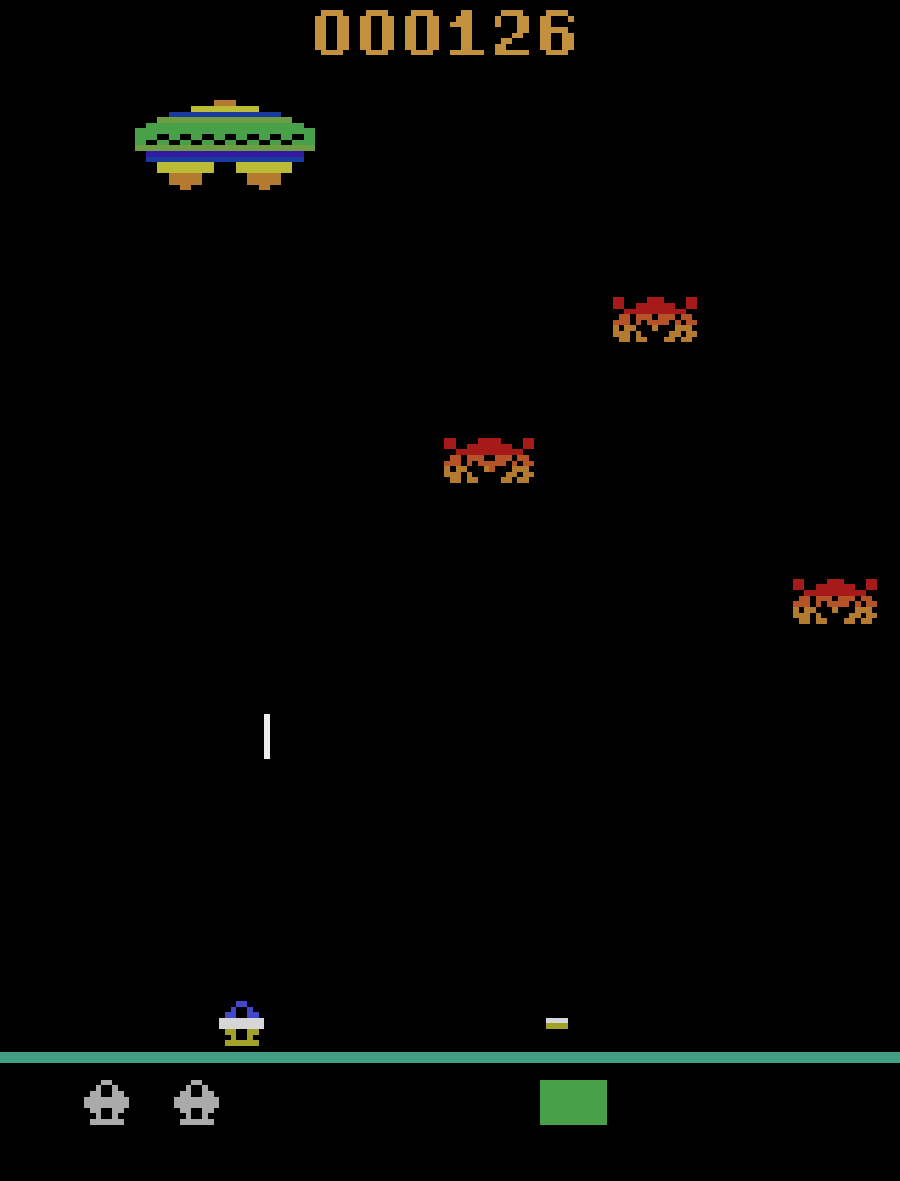
\includegraphics[width=\linewidth]{img/assault_preview.png}
    \caption{Atari Assault env.}
    \label{fig:assault_preview}
  \end{minipage}
\end{wrapfigure}

\textbf{Environment II: Atari Assault.} We consider the Atari game called Assault, where the agent controls a missile launcher to shoot oncoming alien ships while avoiding enemy missiles. The standard approach is to view this as a single-objective environment, where the agent's policy observes the entire image or the 128 byte raw RAM state observations to determine the optimal actions \citep{bellemare13arcade}. 
% This approach lacks transparency and interpretability, because the user will not know why the agent behaved in a certain way. \GS{This is not a good claim.}

For our modular framework, we break the objective down to a multi-objective problem, where each alien ship is viewed as a separate objective, and each local policy attempts to destroy its assigned target while avoiding enemy missiles. 
Not only does this facilitate an improvement in the performance, as we will demonstrate, but also we obtain a transparent design, because which target is being chased is revealed at each point. 
This modular design is made possible by the object-centric variant of the Atari environment \citep{delfosse2023ocatari}, which exposes the states of each individual target and the missiles by decoding the RAM states. 
The full observation space of each local policy also include the current position of the missile launcher, the current health, and the number of remaining lives. 
The local policy gets a reward or a penalty upon destroying its target enemy ship or losing a life, respectively. 
Lastly, we use the game score as the metric for evaluation.


\textbf{Baseline approaches.}
We compare our method against two baselines: a single policy PPO with weighted rewards and deep W-learning (DWN; \citet{rosero2024multi}). 
For the PPO baseline, since all the objectives have the same importance across the two environments, we use the total reward across objectives at each step as the reward function.
We note that in the Atari Assault environment we do not use the game score as a reward and instead use the same rewards perceived by the bidding-based policies to ensure a fair comparison.
The observation space remains the same as the multi-policy setting. 
In the Cat Feeder environment, we implement three reward mechanisms to help guide learning: one only with the sparse rewards from the environment, one with distance-based dense reward with respect to the nearest feeding request (denoted Nearest Shaping/NS in the experiments), and finally one where we provide distance-based reward with respect to the request that has the least amount of time until expiration (denoted Expiry Shaping/ES).
The PPO implementation is taken from CleanRL~\citep{huang2022cleanrl}.
We use the specified PPO hyperparameters from CleanRL for Atari Assault and we tune the hyperparameters for the Cat Feeder environment with 40 Optuna iterations~\citep{akiba2019optuna}.

DWN is another multi-policy method for multi-objective RL that uses DQN for each of the local policies and additionally learns a W-network for each policy that predict scalar weights. 
These weights are used to choose which policy's action should be played at each step. 
The W-network is trained alongside the Q-network by updating it with a gradient step to predict the negative temporal difference (TD) error when the policy does not get to play its action.
The assertion here is that the negative TD-error quantifies how important it is for the policy to play its action. 
The implementation is borrowed from the repository of \citet{rosero2024multi}. All hyperparameters for the baselines are listed in~\Cref{sec:reprod-details}.